%%%%%%%%%%%%%%%%%%%%%%%%%%%%%%%%%%%%%%%%%%%%%%%%%%%%%%%%%
%  PATT2 FORM VERSION 02/2003 - TEMPLATE                %
%%%%%%%%%%%%%%%%%%%%%%%%%%%%%%%%%%%%%%%%%%%%%%%%%%%%%%%%%
%  ENTER THE INFORMATION BETWEEN THE CURLY BRACKETS     %
%%%%%%%%%%%%%%%%%%%%%%%%%%%%%%%%%%%%%%%%%%%%%%%%%%%%%%%%%
%  DO NOT EDIT THE PATT2.STY FILE IN ANY WAY            %
%%%%%%%%%%%%%%%%%%%%%%%%%%%%%%%%%%%%%%%%%%%%%%%%%%%%%%%%%

%%%%%%%%%%%%%%%%%%%%%%%%%%%%%%%%%%%%%%%%%%%%%%%%%%%%%%%%%
% the default font size must not be altered from 11pt.  %
% proposals written in a smaller font will be rejected  %
%%%%%%%%%%%%%%%%%%%%%%%%%%%%%%%%%%%%%%%%%%%%%%%%%%%%%%%%%
                                                       
%\documentstyle[11pt,patt2,epsfig,epsf,psfig]{article} 
\documentclass[11pt]{article}

\usepackage{patt2}
\usepackage{epsfig}
\usepackage{psfig}
\usepackage{epstopdf}
\usepackage{graphicx} 
\usepackage{multirow}
\usepackage{amssymb}


\typeout{This is the PATT2 (Optical/IR) blank LaTeX form}

% add any personal macros here

% end macros

\begin{document}

\telescope{WHT}       % AAT, UKST, WHT, INT or UKIRT
\semester {2019A}    % eg 2003B

\category {5}    % Scientific Category (enter a number):
                % 1 Solar system and extrasolar planets
                % 2 ISM, CSM, PNe, including star formation
                % 3 Stars and stellar populations (galactic and circum-galactic)
                % 4 Low-z universe
                % 5 High-z universe
 
\relatedapps {}{}{}{}{}{}{}{}{} % Coordinated PATT applications {x}
% in order  AAT,UKST,WHT,INT,UKIRT,JCMT,Gemini,LT,MERLIN

%%%%%%%%%%%%%%%%%%%%%%%%
% PAGE 1 OF PATT2 FORM %
%%%%%%%%%%%%%%%%%%%%%%%%

% PI information

\pisurname       {Ross}                
\pititle              {Dr.}                   
\pifirstname     {Nicholas}          
\pistatus          {STFC Ernest Rutherford Fellow}                % Post held
\piaddressone  {Institute for Astronomy}                % Name of Institute
\piaddresstwo  {University of Edinburgh}                % Postal Address
\piaddressthree{Royal Observatory, Blackford Hill}                % Postal Address
\piphone           {+44 (0)131-668 8351}                % Phone number
\pifax                {}                % Fax number
\piemail            {npross@roe.ac.uk}                % email address
\piobserver       {Yes}                % Is the PI going to observe? {Yes/No}


% collaborator 1
\collabonename      {A. Bruce, D.~Homan, A.~Lawrence }             % Name of first collaborator
\collaboneinst         {Univ. Edinburgh}             % Name of Institute
\collaboneobserver {Yes}             % Will collaborator observe? {Yes/No}

% collaborator 2
\collabtwoname     {K.E.S.~Ford, B.~McKernan}
\collabtwoinst        {City University of New York}
\collabtwoobserver {No}

% collaborator 3
\collabthreename    {M.~Graham, D.~Stern}
\collabthreeinst    {California Institute of Technology}
\collabthreeobserver{Yes}

% collaborator 4

\collabfourname    {C.~MacLeod}
\collabfourinst    {Harvard-Smithsonian CfA}
\collabfourobserver{No}

% note additional collaborators can be added by inserting multiple
%names into these entries.



% proposal information 

\title      {Optical Properties of Quasars that have rapidly Rising and Falling Infrared flux}                % Brief title  (12 words only)

\abstract   {
\vspace{-14pt}
``Changing-look'' quasars (CLQs) vary much faster than expected from
classic, thin, Shakura-Sunyaev accretion disks. 
%%
Our team has recently demonstrated that infrared-selected CLQs allow
us to probe the very central regions of quasars, including the
innermost stable circular orbit (ISCO) and potentially test
predictions of General Relativity.
%%
We have extracted a set of 21 IR-selected CLQs from the SDSS using new
data from the NEOWISE-R mission. These objects have striking
falling and rising mid-IR fluxes, but have representative SDSS spectra
from $\approx$6 to 14 years ago (rest-frame). 
%%
We propose the first systematic study of IR-selected CLQs and request 2 dark nights in order to reveal the recent 
optical spectral state of these quasars.
%%
Our baseline expectation is that WHT spectra of the IR Risers (Faders) 
will show hotter, bluer (cooler, redder) disks with larger (smaller) EW broad lines than seen
with SDSS. 
% Likewise, WHT optical spectra of the IR Faders will show cooler, redder disks with smaller EW broad lines than seen by SDSS. 
Any departure from this expectation will further inform us how the 
classical model breaks down. 


% summary of proposed observations
% add your abstract here.  the font size must not be smaller 
% than the default in the style-file
}                


% Instrument requirements

\focalstation          {Cass}                 % eg prime,f/3.3,f/8,f/15,f/36,cs/36
\instrument            {ISIS}                   % eg RGO spec, UCLES, UHRF, Taurus, TTF, IRIS
                                                         % prime focus imager, LDSS etc
\detector                {EEV12/RED+}     % which chip do you want to use?
\gratingsandfilters {R300B+R158R}  % eg UBVRI,H$\alpha$,1200R,etc

\timerequested      {2}{}{}{N}              % No. of {Dark}{Grey}{Bright}{Weeks/Nights/Hours}
\minuseful             {1}{}{}                  % Minimum number of useful {D},{G},{B} 
\lttotaltime            {}{}{}{}                  % For long term proposals indicate the
                                                        % TOTAL requested {D},{G},{B},{W/N/H}

%%%%%%%%%%%%%%%%%%%%%%%%
% PAGE 2 OF PATT2 FORM %
%%%%%%%%%%%%%%%%%%%%%%%%

\prefdates                      {None}   % Preferred dates, eg Jan,Feb
\impossdates                {July}    % Impossible dates, eg Mar,Apr
\datesjustification          {Our targets are setting fast, and there is not ample exposure time between Twilight and very high airmass to obtain our required 
SNR}          % Why impossible? eg wrong RAs, etc
\simultaneous                {}          % Simultaneous with other tels/satellites?
\othertimeconstraints     {}         % eg Moon phase/position,specific dates
\serviceobservingyes      {}         % Observations to be done as Service? {x}
\serviceobservingno       {x}       % or not {x}
\serviceobservingmaybe{}          % or maybe {x}
\supporteverynight    {}              % Support astronomer every night? {x}
\supportnone          {}                 % No support astronomer? {x}
\supportfirstnight    {x}             % Support astronomer first night only? {x}
                                                  % (This is the only option for ING)

% target info                             % Target RA,Dec,Mags,Colours,Exp Time
\targetinfo{
  ID          ~~~~~~ ~~~~   RA (J2000)  ~~~~     Dec (J2000) ~~~~   SDSS $g$-band  ~~  Redshift $z$\\
  {\bf ``Faders''}   (16 in total)                 ~~~~~~ ~~~~                                                                                                             \\
  J1014+0918    ~~~~~~    10:14:15.14 ~~~~~~  +09:18:39.3  ~~~~~~  18.22  ~~~~~~  0.252        \\
  J1028+0600    ~~~~~~    10:28:30.56 ~~~~~~  +06:00:58.4  ~~~~~~  18.57  ~~~~~~  0.312        \\
  J1102+0834    ~~~~~~    11:02:48.02 ~~~~~~  +08:34:04.2  ~~~~~~  18.00  ~~~~~~  0.274       \\
%%  J1137+1852$^{\sharp}$      11:37:51.42   +18:5203.8         0.324                                54180, 2007-Mar-21\\
% % J1204+1702$^{\sharp}$      12:04:47.91   +17:02:56.8        0.298                                54207, 2007-Apr-17  \\
% % J1232+1320                      12:32:15.17   +13:20:32.8          0.286                                53166, 2004-Jun-10 \\
% % J1307$-$0259                   13:07:45.55   $-$02:59:01.        0.307                        51692, 2000-May-28  \\
 % %J1324+0324$^{\sharp}$       13:24:47.64   +03:24:32.6       0.306                            52342, 2002-Mar-09  \\
  %%J1331$-$0249$^{\sharp}$    13:31:51.96   $-$02:49:19.1   0.263                        52426, 2002-Jun-01 \\
  %%J1340+0521$^{\sharp}$        13:40:32.01   +05:21:58.5     0.275                           52373, 2002-Apr-09 \\
  %%J1405+1717$^{\sharp}$        14:05:06.21   +17:17:07.9     0.339                               54509, 2008-Feb-13 \\
  %%J1444+1451$^{\sharp}$        14:44:49.82   +14:51:02.9    0.268                              54234, 2007-May-14  \\
  %%J1447+1759$^{\sharp}$        14:47:21.84   +17:59:06.7    0.302                               54554, 2008-Mar-29    \\   
  %%J1528+1003                        15:28:41.26   +10:03:35          0.328                             53852, 2006-Apr-04  \\
  %%J1535+0119$^{\flat}$           15:35:15.93   +01:19:06.3     0.312                           55358, 2010-Jun-11  \\
  %%J1601+0453                       16:01:03.98   +04:53:27.7        0.262                             53494,  2005-May-04    \\
  %%J1634+1118                      16:34:51.10   +11:18:49.2        0.287                              54585, 2008-Apr-29     \\
%\hline
 {\bf ``Risers'' }(5 objects in total)             ~~~~~~ ~~~~                                                                                       \\
J1211+0103         ~~~~~~        12:11:42.58  ~~~~~~   +01:03:37.1    ~~~~~~   18.46 ~~~~~~   0.293     \\
J1253+1454         ~~~~~~        12:53:27.70  ~~~~~~   +14:54:56.0    ~~~~~~   18.15 ~~~~~~   0.252      \\
J1509+1110         ~~~~~~        15:09:52.19  ~~~~~~  +11:10:47.0     ~~~~~~  18.16  ~~~~~~  0.285  \\
%J1558+1255$^{\sharp}$      15:58:55.34    +12:55:55.2      	  0.288                         54570, 2008-Apr-14 \\
%J1614$-$0110                  16:14:00.30    $-$01:10:06.0        0.253                          51693,  2000-May-29 \\

%enter target information here.  this should include name, ra, dec
%and some indication of magnitude, line flux etc.  it is OK to use
%a small font here.
}

% LIST ALL SIMILAR/SUPPORTING APPLICATIONS TO ANY PATT OR OTHER TIME
% ASSIGNMENT COMMITTEE  
% You must include a brief description of any
% other applications whose targets or science goals are similar to 
% those requested here

\otherapplications{
\begin{tabular}[t]{p{1.6in}p{5.0in}}
%Telescope/Committee & Short title of programme  \\
                                            & \\
PATT: Liverpool Telescope   & 18B,   XPL18A06	PL18B07	P.I. Nicholas P.~Ross, 58.2 hours awarded, B-band \\
                                            & {\it The Optical Monitoring of IR-variable Quasars: New theories, new tests}\\
                                            & \\
PATT: Liverpool Telescope   &  18A,   XPL18A06	PL18A06	P.I. Nicholas P.~Ross, 52 hours awarded, C-band \\
                                           & {\it The Optical Monitoring of IR-variable Quasars: New theories, new tests}\\ 
                                            & \\
                                            &   Both proposals are for optical $ugriz$ monitoring for a sample of 72 quasars with interesting \\
                                           & infrared light curves. This includes the 21 objects here, but no data for our current proposal \\
                                           & were obtained in 2018A. \\
\end{tabular}

}


%%%%%%%%%%%%%%%%%%%%%%%%%%%%%%%%%%%%%%%%%%%%%%%%%%%
% PAGE 3 OF PATT2 FORM - SCIENTIFIC JUSTIFICATION %
%%%%%%%%%%%%%%%%%%%%%%%%%%%%%%%%%%%%%%%%%%%%%%%%%%%

\newcommand{\civ}{C\,{\sc iv}}
\newcommand{\SiIV}{Si\,{\sc iv}}
\newcommand{\mgii}{Mg\,{\sc ii}}
\newcommand{\feii}{Fe\,{\sc ii}}

\sciencecase{
\vspace{2pt}
``Changing-look'' quasars (CLQs) vary much faster than expected from
classic, thin, Shakura-Sunyaev accretion disks, and lead to the
current situation that has been dubbed the ``Quasar viscosity crisis''
where the CLQs have broken standard viscous accretion disk models
([1]). Infrared (IR) observations allow us to rule out obscuration as a
cause of the extreme variability. As we showed in [2] and [3], optical
variability of IR-selected CLQs is so fast and of such large amplitude
that the driver is most likely changes in a puffed-up, viscous inner
accretion disk, close to the innermost stable circular orbit (ISCO).

\smallskip
\smallskip
As a result, IR-selected CLQs ([4] and this proposal) allow us to probe 
the innermost regions of quasars, including the ISCO, the plunging region 
and to investigate predictions of General Relativity in strong gravity.
The role of IR-selection is key to revealing these powerful
probes of disks and spacetime close to the black hole. 

%% Although extreme IR variability rules out the dust obscuration scenario for the currently discovered CLQs, understanding what the {\it hot dust} does, on the outer, or indeed maybe even overlapping, edge of the BLR is crucial to understanding how central engines work and how their photon and energy budget propagate to the nuclear galactic regions.

\smallskip
\smallskip
IR emission from quasars is widely believed to be produced in dusty gas by
reprocessed continuum UV emission. We have extracted a set of
$z\approx 0.3$ quasars that exhibit striking `falling' (Fig.~1; top)
and `rising' (Fig.~1; bottom) mid-IR fluxes over a period of
$\approx$4 years. In each case we have representative SDSS spectra 
(see Fig.~2) from before this fade/rise and we have established that these objects
are not blazars by removing objects that would fulfil a traditional ``radio loud'' 
criterion. 

\smallskip
\smallskip
WHT spectra of these quasars will allow us to carry
out a simple test of the IR ``Risers'' and ``Faders''. Since IR emission
is reprocessed continuum emission from the disk, our baseline
expectation (null hypothesis) is that WHT spectra of the ``Risers'' will
show hotter, bluer disks with larger EW broad lines than seen with
SDSS. Likewise, WHT optical spectra of the ``Faders'' will show cooler,
redder disks with smaller EW broad lines than seen by SDSS. 
%Measuring the EW in both states is good test for SED changes where we need a larger sample than currently available to not be limited statistically.
{\it Here we propose the first ever systematic study of IR-selected
CLQs.  We request two dark nights in order to reveal the optical
spectral properties of these quasars.}

\smallskip
\smallskip
Crucially, we have first epoch spectral data from SDSS, and thus can perform 
an ``absolute'' (i.e. 1st epoch vs. 2nd epoch) measurement as well as a ``relative'' 
(2nd epoch Risers vs. 2nd epoch Faders) test.
%\smallskip \smallskip
By comparing the disk luminosity between the 1st epoch SDSS spectra
and the 2nd epoch WHT spectra we will be able to constrain the change
in the accretion rate and inner disk temperature for each quasar. This
difference should be directly comparable to the magnitude of IR rise
or fall in that quasar between epochs.  Thus, we have a strict and
simple null hypothesis test. A confirmation of the null hypothesis in
our sample gives us some confidence that IR-selection of CLQs is
probing what we think it should, i.e. dusty gas beyond the regular broadline region. 
Any departure from the null hypothesis reveals a flaw in our simple
expectations and a flaw in the IR-selection criterion of CLQs. It will
provide grounds for both follow-up theoretical work and follow-up
observations on a larger sample of risers and faders. The latter
will test the rate of departure from our null hypothesis for CLQs.

\smallskip
\smallskip
%%As such, even if we do not observe any significant differences in the second  spectral epoch to the first, this is {\it deeply interesting} due to the dramatic differences in the associated infrared fluxes. 
%%
%%Moreover, it is currently unknown whether there are any fundamental differences between quasars that show an increase in the MIR flux compared to those that show a decrease. \\

\smallskip
\smallskip
Our sample spans a period of $\approx$6-14 years in the rest-frame
since the SDSS spectra were obtained, see Figure 3, and these objects
also generally have Eddington ratios $\approx$1\% -- 10\%. Calculating if
there has been an increase/decrease in the Eddington ratio in 2019A
will again give key insights on the mechanisms powering extremely
variable quasars.

\smallskip
\smallskip
If our hypothesis is supported by the data, we will be able to
quantify the expected variability in the IR due to optical continuum
changes. This will enable us to further investigate the relationship
between the optical continuum source and the IR source in AGN, and, in
particular how changes of the innermost accretion disk (near the ISCO)
impact AGN structures at parsec (and perhaps larger) scales.

\smallskip
\smallskip
Finally, we note that obtaining time-domain spectroscopy for 
IR-variable quasars, links directly to the WEAVE science 
case and observations of radio AGN and galaxies in the medium 
deep LOFAR surveys and quasars detected in ESA {\it Gaia}.

%See Figure 2. 
%%	WISE J1052+1519 (Stern et al. 2018) and J1100-0053  (Ross et al. 2018) are added at the     end for comparison. 
%{\bf Also}, dust reverberation e.g. Gorjian, Shen, Barth (2017)\\
%Billy Vazquez — Reverberation Mapping of Seyfert 1s: Probing the dusty torus at 3.6 and 4.5 micron with the Spitzer Space Telescope
}

%%%%%%%%%%%%%%%%%%%%%%%%%%%%%%%%%%%%%%%%%%%%%%%%%%%%%%%%
% PAGE 3a OF PATT2 FORM - SCIENTIFIC JUSTIFICATION     %
% FOR PROPOSALS TO AAT, WHT or UKIRT FOR 8 OR MORE     % 
% NIGHTS, AND FOR  ALL (I.E. INCLUDING INT AND UKST)   %
% LONG-TERM AND COORDINATED PROPOSALS (INCLUDING THOSE %
% COORDINATED WITH NON-PATT TELESCOPES)                %
%%%%%%%%%%%%%%%%%%%%%%%%%%%%%%%%%%%%%%%%%%%%%%%%%%%%%%%%

\extendedsciencecase{

% continue your science case here ONLY if applying for 8 or 
% more nights to the AAT, WHT OR UKIRT, or if your proposal 
% is a long-term (multi-semester) proposal to the AAT, UKST, 
% WHT, INT or UKIRT, or if your proposal (to AAT, UKST, WHT, 
% INT or UKIRT) is coordinated with other telescopes (including 
% non-PATT telescopes).  

% Remember to comment IN the \makepatttwopagethreea command later 
% in this file if you have written an extended science case  

% proposals written in a font smaller than 11pt will be rejected

}


%%%%%%%%%%%%%%%%%%%%%%%%%%%%%%%%%%%%%%%%%%%%%%%%%%%%%%%%%%%%%%%%%%%%%%%%%%%%
% PAGE 4 OF PATT2 FORM - TECHNICAL INFORMATION (I) - FEASIBILITY, S/N, ETC %
%%%%%%%%%%%%%%%%%%%%%%%%%%%%%%%%%%%%%%%%%%%%%%%%%%%%%%%%%%%%%%%%%%%%%%%%%%%%

\technicalpage{

\vskip 0.1cm
Our proposal is to obtain new spectroscopic epochs for 21 objects that
have been identified due to their startling rising or falling mid-infrared light curves. 

\vskip 0.2cm
{\bf Sample construction.} Take SDSS DR14Q (P{\^a}ris et al., 2018,
A\&A, 613A, 51; 526,356 quasars) and limit to $0.25 \leq z \leq
0.35$ in order to access \mgii, H$\beta$ and H$\alpha$ in WHT/ISIS
spectra; sample drops to 3193 quasars.  For this redshift range,
WISE W1 (W2) accesses rest-frame 2.52-2.72 (3.33-3.60) $\mu$m, so
still corresponding to hot dust.  Limit to Decl. $\delta \leq +20$
deg to enable follow-up from Southern Hemisphere; sample drops to
1233 quasars.  Obtain the NEOWISE-R 2018DR light curves, and apply
additional requirement that $w1snr>2$ for individual L1b frames;
sample drops to 1219 quasars.  Visually inspect all 1219 NEOWISE-R light
curves for interesting objects (i.e., quasars with obviously rising
or fading NEOWISE-R light curves) and concentrate on objects with
$120 < R.A./deg < 250$ for 2019A.  This yields a sample of 23 objects
(17 ``Faders'', 6 ``Risers'').

\smallskip
\smallskip
We then checked for blazars via the CRATES Flat-Spectrum Radio
Source Catalog (heasarc.gsfc.nasa.gov/W3Browse/radio-catalog/crates.html),
finding no matches.  We also checked with VLA FIRST Catalog Database
(2014dec17) and removed two objects, one with a FIRST detection,
and one radio-undetected source that might fit the
radio-to-optical flux ratio definition of radio-loud (e.g., Stern
et al., 2000, AJ, 132, 1526)  given its faint optical magnitude.
{\bf We arrive at a sample of 21 objects with 16 of these being 
``Faders'' and 5 being ``Risers''.}

%\vskip 0.2cm
%{\bf Experimental Procedure:} 

\vskip 0.2cm
{\bf Observing Notes:} 
Our sample of 21 targets ranges from $g = 16.97-19.30$ mags, though 
all but two are brighter than $g=18.97$ mag from their SDSS photometry. 
The sample naturally breaks down into a ``Bright'' $g<18.5$ subsample with 13 objects 
and a ``Fainter'' subsample with 8 objects having $18.50<g<19.30$. 

\vskip 0.2cm
{\bf Time requirement.}  
Based on recent experience (with the CLQ sample in 16A/17A), and given
the estimated $g$-band magnitudes of these objects, we estimate
2$\times$450sec science exposures for our Bright subsample (for a
total of 900sec$\times$13=11,700secs) and 2$\times$900sec science
exposure for our ``Fainter'' sample (for a 1800sec$\times$8=14,400secs)
for a 26,100sec = 7.25 hours total science exposure time.
Given these exposure times, our past experience, and values from SIGNAL
(1.00'' seeing, 1.20 airmass, 1.00'' slit width, Dark time) we 
achieve, SNR of $\approx$10-20/pixel for all our targets.  
We {\it nota bene} that {\it if} any of our objects have faded in the optical 
to the extent that these exposure times are {\it not} sufficient, that in of 
itself is a key discovery and fascinating result.

\smallskip
\smallskip
With this Total Science Exposure time and including all the ISIS
overheads using the TOTE (42 telescope pointings; 21 autoguiding
preparations; 21 object acquisitions: 42 detector readouts; 2 changes
of grating, no changes of the dichroic and 22 spectroscopic arcs) we
 have a {\bf total estimated time of 43,424 sec = 12:06 hours and 
therefore request two full Dark nights.}  We require Dark Time in
order to maximise SNR in the blue and in particular for the \mgii\ line, 
continuum slope and SED measurements.  {\it At a minimum, we request 1.00 dark
night to observe 8-10 targets, e.g. the full ``Risers'' sample and an
equivalent number of ``Faders''.}

\vskip 0.2cm
{\bf Spectroscopic set up.} 
WHT+ISIS is the ideal instrument as has been repeatedly demonstrated
on our previous observing runs.  The sensitivity and wide wavelength
coverage with the two arms is essential for detecting \mgii, H$\beta$
and H$\alpha$ over the redshift range of the targets ($z=0.25$--0.35).
Indeed, our redshift range is specifically chosen so that WHT+ISIS
can access these broadlines.

\smallskip
\smallskip
We need medium resolution so that the broadlines are well
resolved, and ideally so that the narrow lines (width $\sim 500$ km/s)
are at least marginally resolved. We use grating R300B in the blue
arm, with 0.86\AA /pixel, and with a 1$^{\prime\prime}$ slit giving
resolution 3.4\AA , equivalent to velocity resolution of 200km/s at
5200\AA . With the red arm we use R158R which gives a similar velocity
resolution at 7000\AA.  This combination gives complete wavelength
coverage with reasonable resolution. 

%\smallskip \smallskip
%As with our previous observations, we will use the 5300 dichroic along with the R158B and R300B gratings 
%in the red and blue arms, respectively. The GG495 order sorting filter in the red arm is typically used and 
%2× binning is usually performed in the spatial direction. 


%%  EEV12   /  RED+
%%  R300B  +  R158R
%% Relatively bright (g < 20.5) and highly variable (|∆g| > 1.3 mag) CLQ candidates were observed on February 6-8 and May 30, 31 2016 using the 4.2m William Herschel Telescope (WHT) in La Palma. Observations were performed using the Intermediate dispersion Spectrograph and Imaging System (ISIS). The 5300 dichroic was used along with the R158B and R300B gratings in the red and blue arms, respectively, along with the GG495 order sorting filter in the red arm. Typically 2× binning in the spatial direction was used to improve the signal-to-noise ratio (SNR) along with a narrow CCD window to reduce memory usage and readout times. This set-up gives a spectral resolution of R ∼1500  ̊  ̊ ′′  ̊ at 5200 A in the blue and R ∼1000 at 7200 A in the red for a slit width of 1. 0 and total coverage ∼ 3100–10600 A. Typically, calibration images were taken at the start of each night including bias frames, lamp flats and CuNe/Ar arc lamp images. Spectroscopic standard stars were observed at ∼2h intervals throughout the night though this cadence was not always possible. Observations were carried out at the parallactic angle. Exposures were taken in 1800s increments and the number of shots on target was adjusted based on the latest PS1 photometry. WHT data were reduced using custom pyraf scripts and standard techniques.



% add any technical details you wish to transmit to the panel and
% technical assessor here. you may also include references here
% as well as on the next page

% proposals written in a font smaller than 11pt will be rejected
}


%%%%%%%%%%%%%%%%%%%%%%%%%%%%%%%%%%%%%%%%%%%%%%%%%%%%%%%%%%%%%%%%%%%%%%%%%%%%%%
% PAGE 4a OF PATT2 FORM - TECHNICAL INFORMATION (II) - REFERENCES, FIGS, ETC %
%%%%%%%%%%%%%%%%%%%%%%%%%%%%%%%%%%%%%%%%%%%%%%%%%%%%%%%%%%%%%%%%%%%%%%%%%%%%%%

\figsandrefspage{

%\vspace{-.2cm}
%\begin{figure}
%\centering
%\includegraphics[width=12.5cm, angle=0]{Fig1.pdf}
%\caption{ {\bf Figure 1:} }
%\end{figure}

%\includegraphics[width=8.5cm, angle=0]{2019A_figures/Stern_2018_ApJ_Figure1.pdf}
%\includegraphics[width=8.5cm, angle=0]{2019A_figures/Stern_2018_ApJ_Figure1.pdf}

\includegraphics[width=18.5cm, height=5.4cm ]{2019A_figures/NEOWISER_LCs_3panels_SingleObjects_Faders.pdf}
\vspace{12pt}
\includegraphics[width=18.5cm, height=5.4cm]{2019A_figures/NEOWISER_LCs_3panels_SingleObjects_Risers.pdf}

%If you still have problems, then add these two other packages at the beginning of your document for a correct invocation, after \do
{\bf Figure 1:} The NEOWISER light curves of the first three ``Faders'' and first three ``Risers'' in our target list. These data are typical of our sample and show very clear and dramatic changes in 3.4$\mu$m W1 and 4.6$\mu$m W2 flux. 

%{\bf Figure 2:} 
\centering
\includegraphics[width=16.5cm]{2019A_figures/Figures2_and_Figure3.pdf}
%\centering
%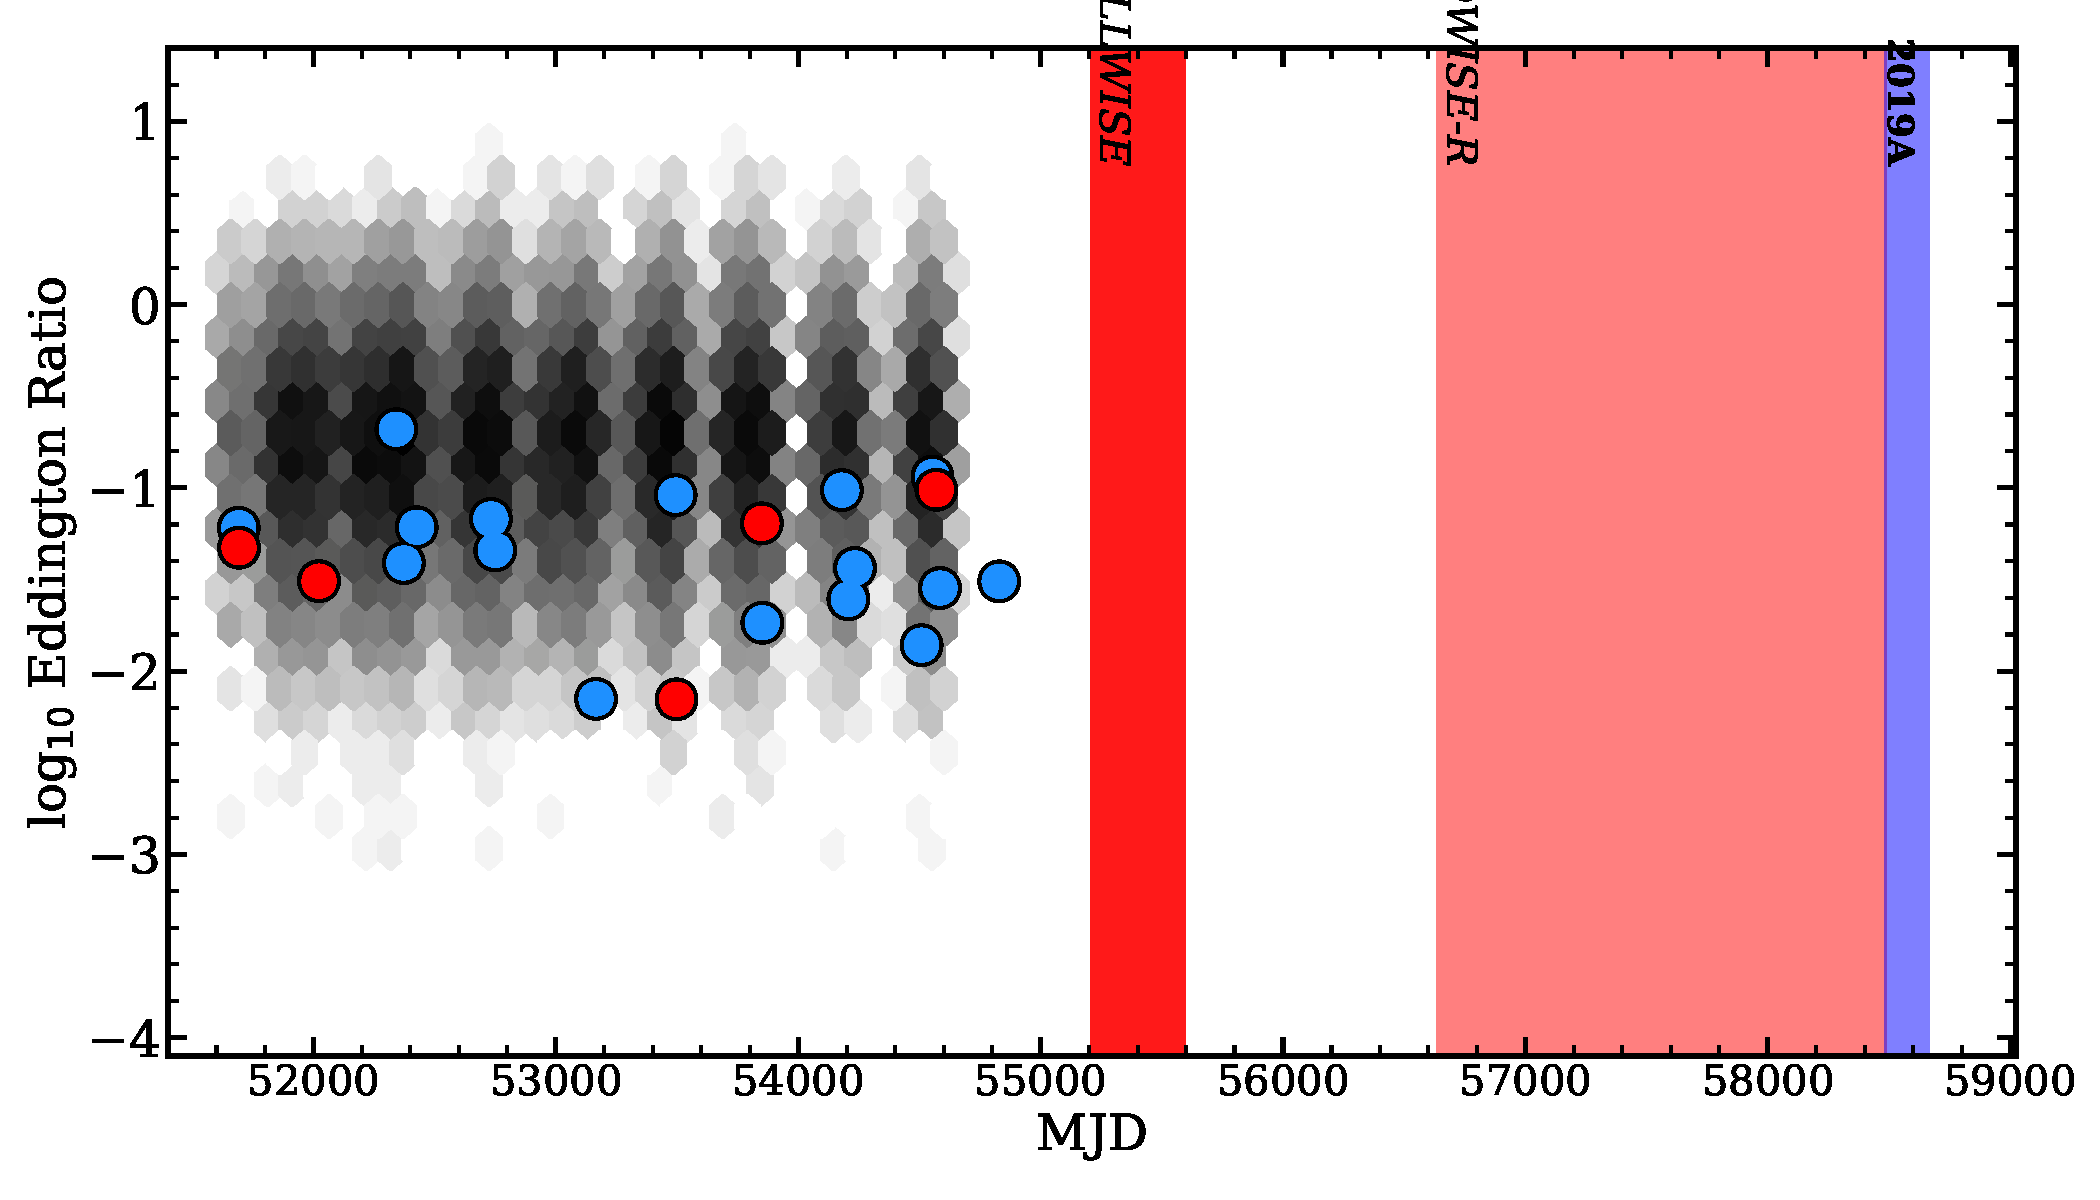
\includegraphics[width=6.5cm, height=9.0cm]{MJD_Eddington/MJD_vs_Eddington_temp.pdf}

%\begin{minipage}[b]{0.4\textwidth}
 %   \includegraphics[width=\textwidth]{2019_spectra_fig/Risers_and_Faders_v1.pdf}
%    \caption{Flower one.}
 % \end{minipage}
  %\hfill
  %\begin{minipage}[b]{0.4\textwidth}
    %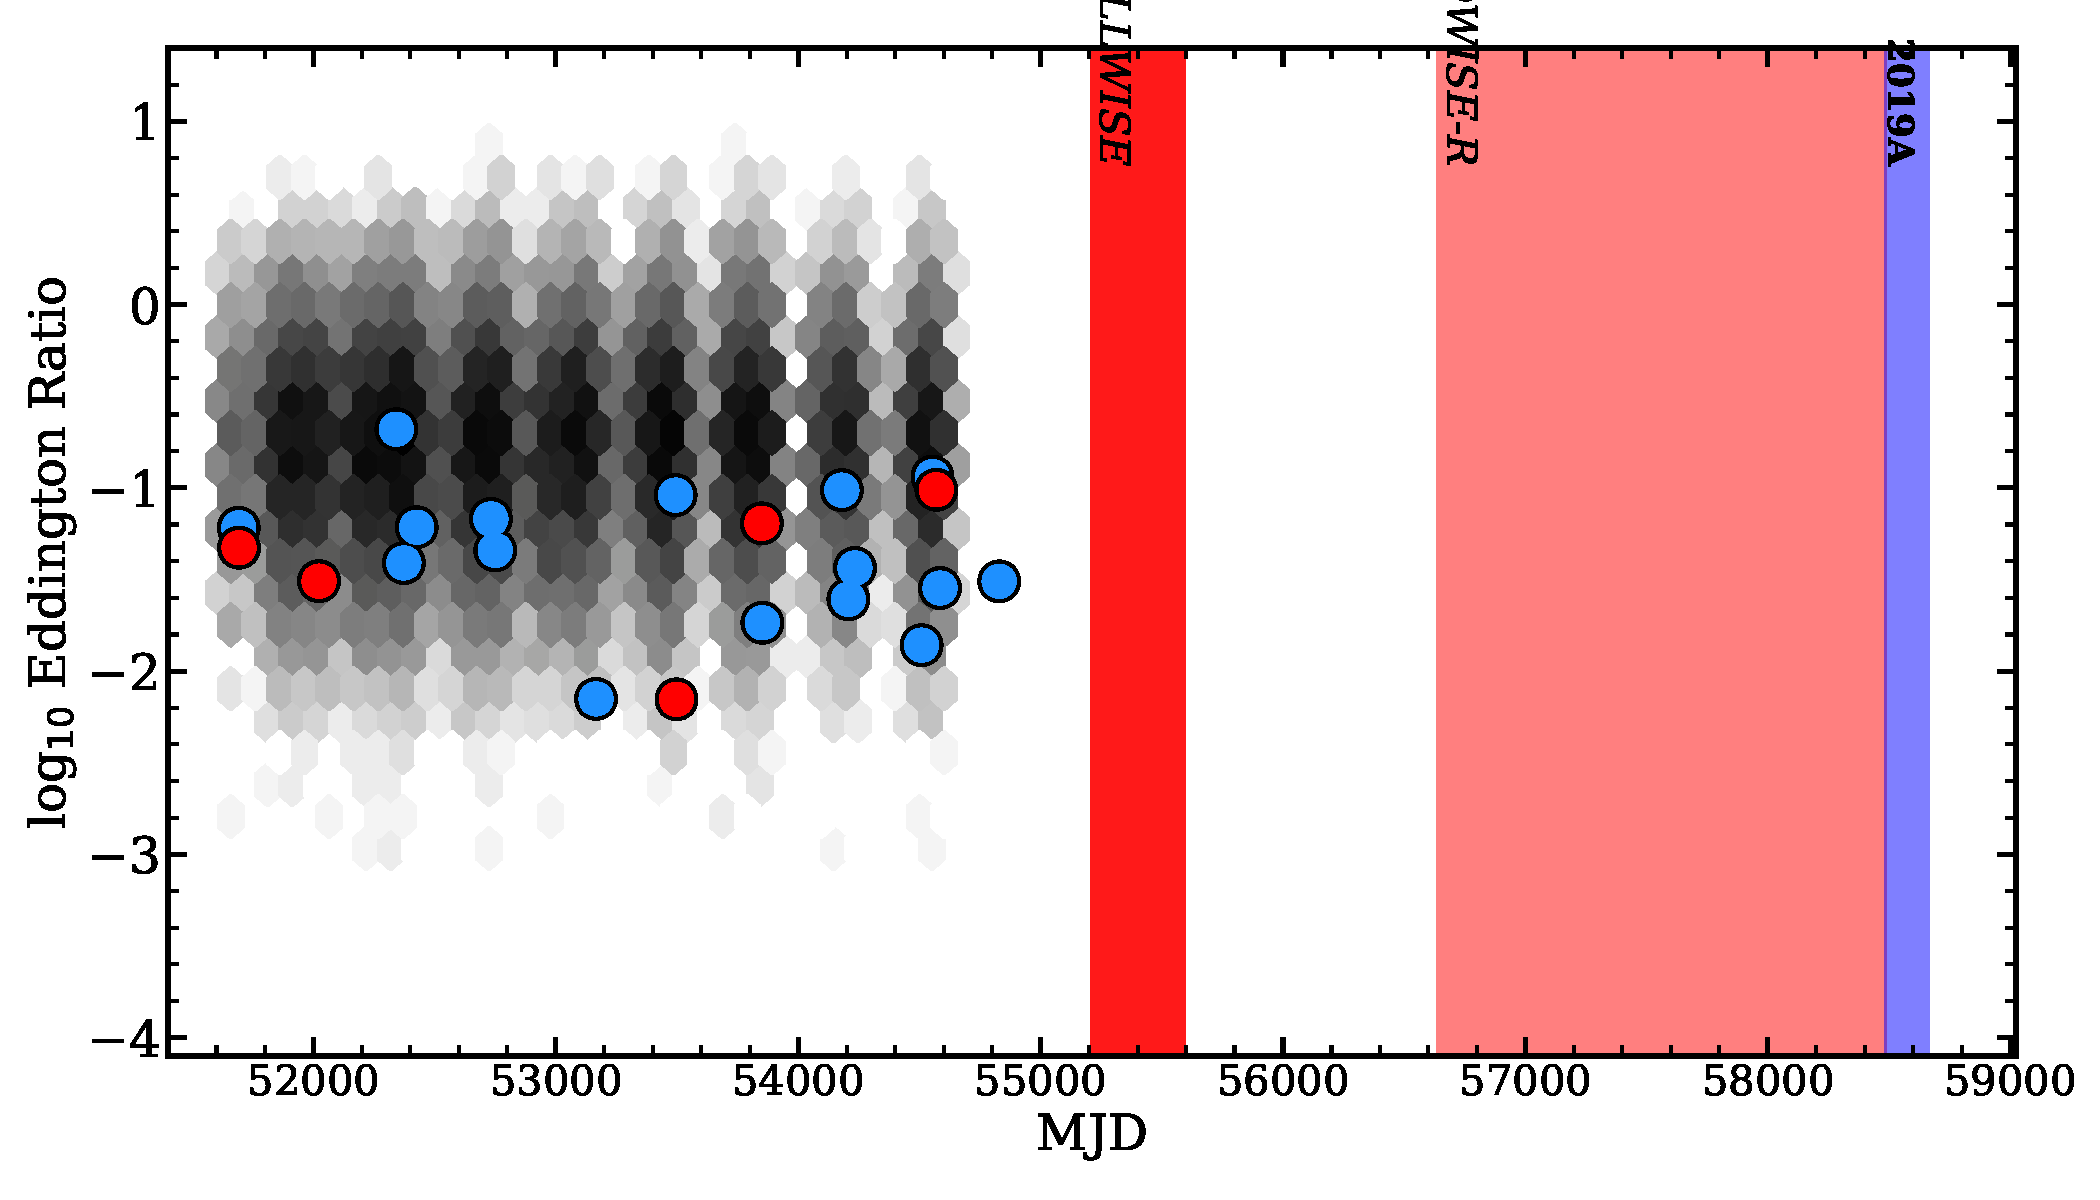
\includegraphics[width=\textwidth]{MJD_Eddington/MJD_vs_Eddington_temp.pdf}
%    \caption{Flower two.}
 % \end{minipage}

\vspace{-42pt}

\parbox{22.0cm}
{
\small  
%\footnotesize \scriptsize %\tiny
{\bf References:} \\
\lbrack1\rbrack Lawrence, 2018, NatAs, 2, 102 \\
\lbrack2\rbrack Stern et al. 2018, ApJ, 864, 27;  \\
\lbrack3\rbrack Ross et al., 2018, MNRAS, 480, 4468 \\
\lbrack4\rbrack Graham et al. 2018, ApJ; in advanced prep.\\
\lbrack5\rbrack P{\^a}ris et al., 2018, A\&A, 613A, 51 \\
\lbrack5\rbrack Stern et al., 2000, AJ, 132, 1526\\
%\lbrack5\rbrack Yang et al. 2018, ApJ, 862, 109\\
%\lbrack6\rbrack Sheng et al, 2017, ApJL, 846, L7


}
% add any figures, references etc here.  remember to embed your figures.
% you can only use epsf or psfig to embed figures.

% proposals written in a font smaller than 11pt will be rejected
}


%%%%%%%%%%%%%%%%%%%%%%%%
% PAGE 5 OF PATT2 FORM %
%%%%%%%%%%%%%%%%%%%%%%%%

\backupprogram{}             % Summary of backup programme

\previous{                   % Previous applications (last 4 Sems)
  \begin{tabular}[t]{p{1.5in}p{0.7in}p{0.8in}p{3.2in}}
    % Patt No. & Award & clear nights & comments \\
%    LT PATT:   & & & \\
    LT 18A/B:  	PL18A08  &	B	14h      & & "Continued reduced cadence monitoring of large amplitude microlensing events"\\
    LT 17A/B:  	PL17A09 &       A	21h      & & "Continued monitoring programme for high-value, slow, smooth AGN hypervariables"\\
%&&&\\
%    WHT PATT: &&&\\
    WHT  17A/B:  & 	 	2D2G (17A)       &  & Continuing: SW2017b05   "Mapping the transverse \\
                                            &   1D1G+    & &          structure of the BLR and torus in hypervariable AGN"	\\
                                            &    1DS1GS (17B)       & &		 \\
\end{tabular}
}

\publications     {
\vspace{2pt}
Bruce, A., Lawrence, A., MacLeod, C., et al. 2017, MNRAS, 467, 1259\\
Collinson et al. (incl. Lawrence, Bruce, MacLeod), 2018, MNRAS, 474, 3565\\
Kankare, E. (incl. Lawrence, Bruce), Nature Astronomy, 1, 865\\
MacLeod et al (2018), ApJ, collaboration submitted. \\
}         % List pubs with data from patt time (last 4 Sems)

\experience       {All proposers experienced WHT observers except Ross, who is an experienced user of AAT and similar US telescopes} 
                          %  Experience of observers on other telescopes
\graduatestudent  {}{}       % Research student {Name of student}{Project}
\grant            {N.P. Ross}{STFC Ernest Rutherford Fellowship}{}     % {Name of PI}{Grant title}{Grant No.} 
\nonstandardtravel{}         % Justify T&S for more than one UK observer
\otherexpenditure {}         % eg for freight etc.


%%%%%%%%%%%%%%%%%%%%%%%%%%%%%%%%%%%%%%%%%%%%%%%%%%%%%%%%%%%%%%%%%%%%%%%%%%%%%
% PAGE 6 OF PATT2 FORM - THIS SECTION IS REMOVED BY THE AAT DURING PROCESSING
% IF INCLUDED.  ING APPLICANTS SHOULD NOT ENTER ANYTHING HERE.
%%%%%%%%%%%%%%%%%%%%%%%%%%%%%%%%%%%%%%%%%%%%%%%%%%%%%%%%%%%%%%%%%%%%%%%%%%%%%

\shorttitle {}              % Ignore if you are an ING applicant.


\makepatttwopageone
\makepatttwopagetwo
\makepatttwopagethree

%%%%%%%%%%%%%%%%%%%%%%%%%%%%%%%%%%%%%%%%%%%%%%%%%%%%%%%%%%%%%%%%%%%%%
% COMMENT THE FOLLOWING LINE IN *ONLY* IF                           % 
%                                                                   %
% YOU ARE APPLYING FOR 8 OR MORE NIGHTS ON THE AAT, WHT OR UKIRT, OR% 
% YOUR PROPOSAL IS LONG-TERM FOR THE AAT, WHT, UKIRT OR INT, OR     % 
% YOUR PROPOSAL IS COORDINATED WITH OTHER TELESCOPES                % 
%                                                                   % 
% *AND* YOU HAVE USED THE CONTINUATION PAGE FOR YOUR SCIENTIFIC CASE% 
%%%%%%%%%%%%%%%%%%%%%%%%%%%%%%%%%%%%%%%%%%%%%%%%%%%%%%%%%%%%%%%%%%%%%
 
%\makepatttwopagethreea

\makepatttwopagefour
\makepatttwopagefoura
\makepatttwopagefive

% FOR ING APPLICATIONS LEAVE THE FOLLOWING LINE COMMENTED OUT

%\makepatttwopagesix         

% FOR AAT APPLICATIONS YOU MAY LEAVE IT IN IF YOU WISH.  IT WILL NOT
% BE TRANSMITTED TO THE TAG HOWEVER.

\end{document}
